\documentclass[a4paper,11pt]{article}

\usepackage [french]{babel}
\usepackage [utf8]{inputenc}
\usepackage{graphicx}
\usepackage[T1]{fontenc}
\usepackage{textcomp}
\usepackage{vmargin}
\usepackage{dirtree}
\usepackage{listingsutf8}
\usepackage{xcolor}
\usepackage{textcomp}
\usepackage{float}
\usepackage{hyperref}
\usepackage{fancyhdr}
%\usepackage{fullpage}

\begin{document}

\lstset{
  inputencoding=utf8/latin1,
  belowcaptionskip=1\baselineskip,
  inputencoding=utf8/latin1,
  breaklines=true,
  language=C++,
  showstringspaces=false,
  basicstyle=\footnotesize\ttfamily,
  keywordstyle=\bfseries\color{purple!40!black},
  commentstyle=\itshape\color{green!40!black},
  identifierstyle=\color{black},
  stringstyle=\color{blue},
  morekeywords={QXmlStreamReader, QString, QTextCursor, QSyntaxHighLighter, QRegExp, XmlFileManager, QFile, QIODevice, QDomNode, QDomDocument, stack, ModeleXml, QStandardItem, QStandardItemModel, QModelIndex},
    showspaces=false,                % show spaces everywhere adding particular underscores; it overrides 'showstringspaces'
  showtabs=false,                  % show tabs within strings adding particular underscores
  stepnumber=2,                    % the step between two line-numbers. If it's 1, each line wil
  tabsize=2,                       % sets default tabsize to 2 spaces
  frame=lrtb,
  numbers=left
}

\title{\textbf{Imagerie 3D}\\Compte rendu TP1}
\author{\textit{\date\today Stéphane Wouters}}

\maketitle
\thispagestyle{empty}

\newpage 

\tableofcontents

\newpage 

\section{Stockage de l'image}
\paragraph{}

{\bf Méthode:} Utilisation d'une classe Image. Stockage dans un tableau binaire linaire, puis lecture via des calculs sur les indexes.

\paragraph{}


Tableau utilisé : \textit{VALUE* bin;}
\\
Avec un \textit{typedef unsigned short VALUE;}

\subsection{Lecture de l'image}

L'image lue est entièrement stockée dans le tableau.

\begin{lstlisting}
void load(char* filename) {
	FILE *f_image;

	if ((f_image = fopen(filename, "rb")) == NULL) {
		printf("\nErreur lecture %s \n", filename);
		exit(EXIT_FAILURE);
	}
	else {
		if (fread((VALUE*)bin, sizeof(VALUE), getSize(), f_image) != 
			(size_t)(getSize()))
		{
			printf("\nErrur lecture %s \n", filename);
			exit(EXIT_FAILURE);
		}
		fclose(f_image);
	}
}
\end{lstlisting}

\subsection{Accès à une valeur x,y,z}

L'accès à une valeur se fait par un calcul de dimension sur le tableau.

\begin{lstlisting}
// Pour recuperer la valeur finale
VALUE getValue(int x, int y, int z) {
	return convertValue(*getVoxel(x,y,z));
}

// Convertion double octet
VALUE convertValue(VALUE v) {
	int x1 = v/256;
	int x2 = v - x1*256;
	return x2*256 + x1;
}

// Recuperer un poiteur vers le voxel
VALUE* getVoxel(int x, int y, int z) {
	return &bin[getIndexInTabBin(x,y,z)];
}

// Calcul d'exploration
int getIndexInTabBin(int x, int y, int z) {
	int v = z*sizeX*sizeY + y*sizeX + x;
	return v;
}
\end{lstlisting}

\subsection{Définition d'une valeur}

\begin{lstlisting}
void setValue(int x, int y, int z, VALUE val) {
	*getVoxel(x,y,z) = convertValue(val);
}
\end{lstlisting}

\section{Application}

On test la classe en récupérant des valeurs de certains pixels, ainsi que les valeurs maximums et minimums.

\begin{lstlisting}
Image in(448,576,72);
char path[250] = "beaufix.448x576x72.0.6250x0.6250x1.4.img";
in.load(path);
cout << "minValue = " << in.getMinValue() << endl;
cout << "maxValue = " << in.getMaxValue() << endl;
cout << "value = " << in.getValue(200,200,20) << endl;
\end{lstlisting}

On retrouve les valeurs spécifiés dans la feuille de TP.

\begin{itemize}
  \item minValue = 0
  \item maxValue = 334
  \item l(200,200,20) = 14
\end{itemize}

\section{Volume rendering}
Pour calculer le volume rendering ; On crée une nouvelle image, puis on écrit sur la même couche numéro 0 le résultat du calcul appliqué sur toutes les couches en fonction de l'algorithme

\subsection{Algorithme MinIP}
\begin{lstlisting}
for (int i = 0; i < in.sizeX; ++i)
	for (int j = 0; j < in.sizeY; ++j) {
		VALUE minVal = in.getValue(i,j,0);
		for (int k = 0; k < in.sizeZ; ++k) {
			minVal = min(in.getValue(i,j,k), minVal);
		}
		out.setValue(i,j,0,minVal);
	}
\end{lstlisting}

\subsection{Algorithme MIP}
\begin{lstlisting}
for (int i = 0; i < in.sizeX; ++i)
	for (int j = 0; j < in.sizeY; ++j) {
		VALUE maxVal = in.getValue(i,j,0);
		for (int k = 0; k < in.sizeZ; ++k) {
			maxVal = max(in.getValue(i,j,k), maxVal);
		}
		out.setValue(i,j,0, maxVal);
	}
\end{lstlisting}

\subsection{Algorithme AIP}
\begin{lstlisting}
for (int i = 0; i < in.sizeX; ++i)
	for (int j = 0; j < in.sizeY; ++j) {
		unsigned long long val = 0;
		for (int k = 0; k < in.sizeZ; ++k) {
			val += in.getValue(i,j,k);
		}
		out.setValue(i,j,0,val/in.sizeZ);
	}
\end{lstlisting}

\section{Résultats}

\begin{figure}[[!h]
	\begin{minipage}[c]{.22\linewidth}
     \center
	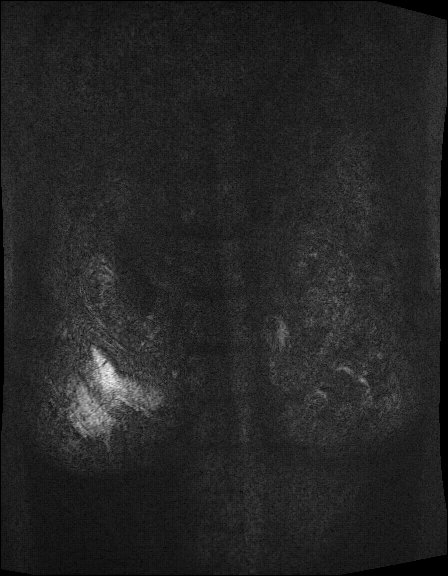
\includegraphics[scale=0.26]{beaufix_MinIP.jpg}
	\caption{Beaufix MinIP}
   \end{minipage} \hfill
	\begin{minipage}[c]{.22\linewidth}
      \center
	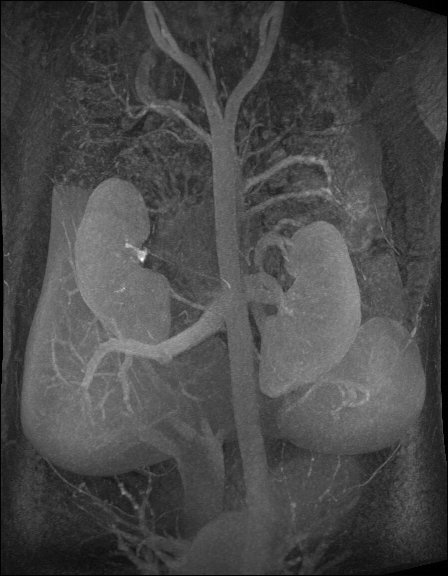
\includegraphics[scale=0.26]{beaufix_MIP.jpg}
	\caption{Beaufix MIP}
   \end{minipage} \hfill
   \begin{minipage}[c]{.22\linewidth}
      \center
	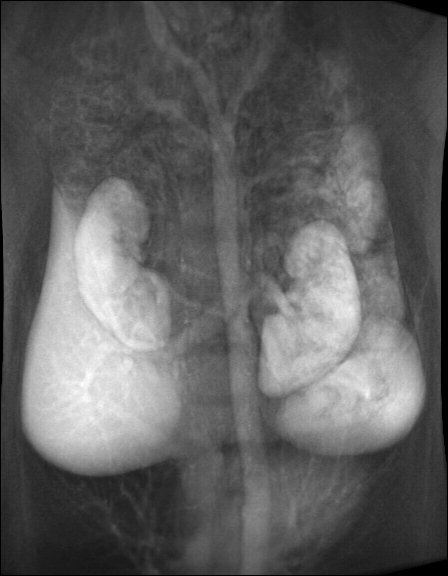
\includegraphics[scale=0.26]{beaufix_AIP.jpg}
	\caption{Beaufix AIP}
   \end{minipage} \hfill
\end{figure}

\begin{figure}[!h]
	\begin{minipage}[c]{.22\linewidth}
     \center
	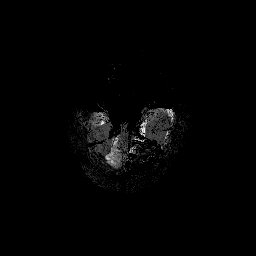
\includegraphics[scale=0.5]{brainix_MinIP.jpg}
	\caption{Brainix MinIP}
   \end{minipage} \hfill
	\begin{minipage}[c]{.22\linewidth}
      \center
	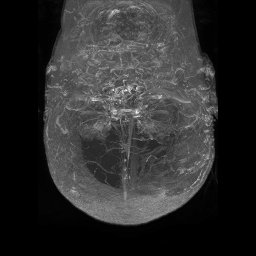
\includegraphics[scale=0.5]{brainix_MIP.jpg}
	\caption{Brainix MIP}
   \end{minipage} \hfill
   \begin{minipage}[c]{.22\linewidth}
      \center
	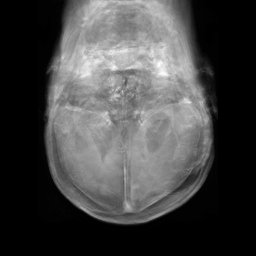
\includegraphics[scale=0.5]{brainix_AIP.jpg}
	\caption{Brainix AIP}
   \end{minipage} \hfill
\end{figure}

\begin{figure}[!h]
	\begin{minipage}[c]{.22\linewidth}
     \center
	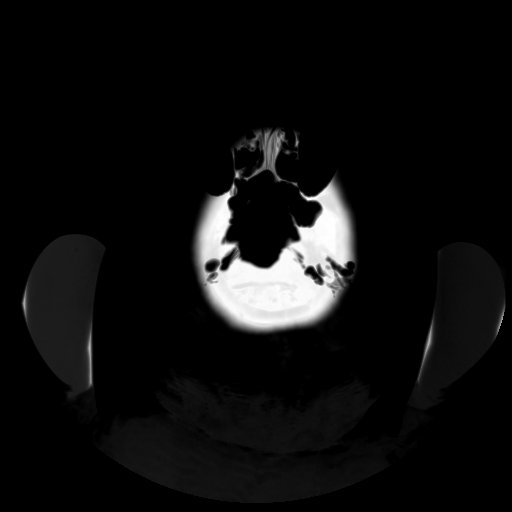
\includegraphics[scale=0.25]{manix_MinIP.jpg}
	\caption{Manix MinIP}
   \end{minipage} \hfill
	\begin{minipage}[c]{.22\linewidth}
      \center
	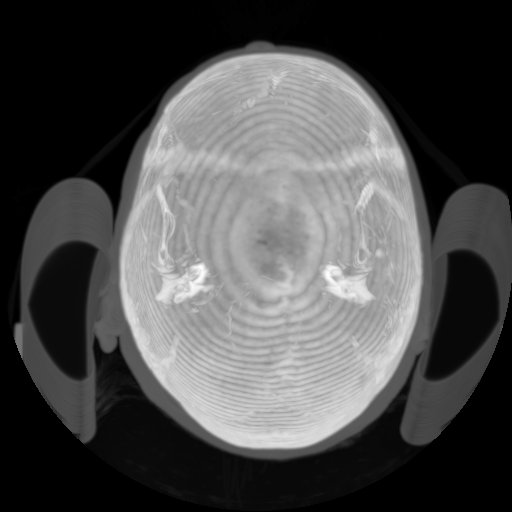
\includegraphics[scale=0.25]{manix_MIP.jpg}
	\caption{Manix MIP}
   \end{minipage} \hfill
   \begin{minipage}[c]{.22\linewidth}
      \center
	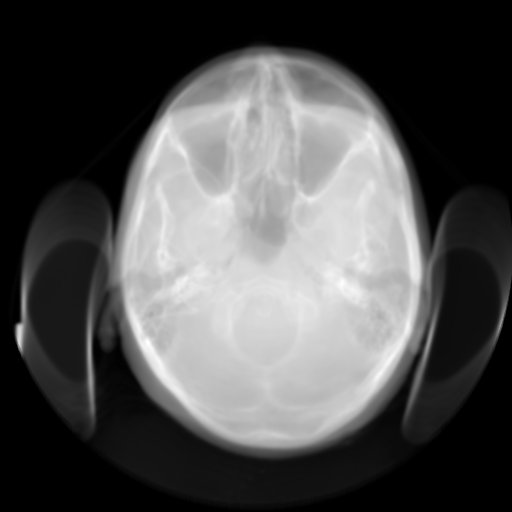
\includegraphics[scale=0.25]{manix_AIP.jpg}
	\caption{Manix AIP}
   \end{minipage} \hfill
\end{figure}

\begin{figure}[!h]
	\begin{minipage}[c]{.42\linewidth}
     \center
	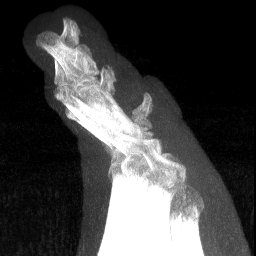
\includegraphics[scale=0.5]{foot_MIP.jpg}
	\caption{Foot MIP}
   \end{minipage} \hfill
	\begin{minipage}[c]{.42\linewidth}
      \center
	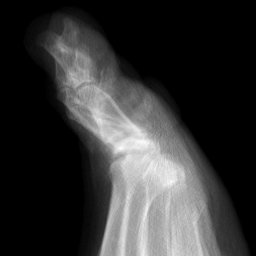
\includegraphics[scale=0.5]{foot_AIP.jpg}
	\caption{Foot AIP}
   \end{minipage} \hfill
\end{figure}

\paragraph{}
\paragraph{}

\section{What is it ?}

\paragraph{}
Avec l'algorithme AIP et en spécifiant au logiciel la taille de l'image, on obtient ceci :

\begin{figure}[!h]
 \center
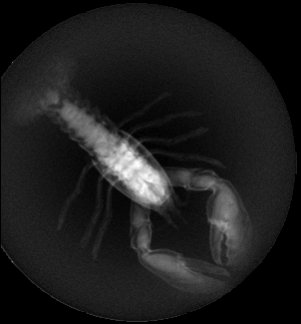
\includegraphics[scale=0.7]{whatisit.jpg}
\caption{Whatisit AIP}
\end{figure}

\section{Code source}
\subsection{Librairie Image}

\begin{lstlisting}
#ifndef IMAGE_PPM
#define IMAGE_PPM

#include <iostream>
#include <stdlib.h>
#include <stdio.h>
#include <string.h>
#include <math.h>

typedef unsigned short VALUE;

class Image {

private:

	VALUE* bin;

	void allocateValues() {
		bin = new VALUE[getSize()];	
	}

	int getSize() {
		return sizeX*sizeY*sizeZ;
	}

	void testValue(int x, int y, int z) {
		if (x > sizeX) {
			printf("L'indice se trouve en dehors des limites de l'image (x %d > %d)\n", x, sizeX);
			exit(0);
		}
		if (y > sizeY) {
			printf("L'indice se trouve en dehors des limites de l'image (y %d > %d)\n", y, sizeY);
			exit(0);
		}
		if (z > sizeZ) {
			printf("L'indice se trouve en dehors des limites de l'image (z %d > %d)\n", z, sizeZ);
			exit(0);
		}
	}

	VALUE convertValue(VALUE v) {
		int x1 = v/256;
		int x2 = v - x1*256;
		return x2*256 + x1;
	}

	VALUE unconvertValue(VALUE v) {
		return convertValue(v);
	}

	int getIndexInTabBin(int x, int y, int z) {
		int v = z*sizeX*sizeY + y*sizeX + x;
		return v;
	}

	VALUE* getVoxel(int x, int y, int z) {
		return &bin[getIndexInTabBin(x,y,z)];
	}

public:
	
	int sizeX; // Largeur
	int sizeY; // Hateur
	int sizeZ; // Profondeur
	
	Image(int sizeX, int sizeY, int sizeZ) {
		this->sizeX = sizeX;
		this->sizeY = sizeY;
		this->sizeZ = sizeZ;
		this->allocateValues();
	}

	VALUE getValue(int x, int y, int z) {
		return convertValue(*getVoxel(x,y,z));
	}

	void setValue(int x, int y, int z, VALUE val) {
		*getVoxel(x,y,z) = unconvertValue(val);
	}

	VALUE getMinValue() {
		int min = bin[0];
		for (int i = 0; i < getSize(); ++i) {
			int v = this->convertValue(bin[i]);
			if (v < min)
				min = v;
		}
		return min;
	}

	VALUE getMaxValue() {
		int max = bin[0];
		for (int i = 0; i < getSize(); ++i) {
			int v = this->convertValue(bin[i]);
			if (v > max)
				max = v;
		}
		return max;
	}

	void load(const char* filename) {
		FILE *f_image;

		if ((f_image = fopen(filename, "rb")) == NULL) {
			printf("\nPas d'acces en lecture sur l'image %s \n", filename);
			exit(EXIT_FAILURE);
		}
		else {
			if (fread((VALUE*)bin, sizeof(VALUE), getSize(), f_image) != (size_t)(getSize())) {
				printf("\nErreur de lecture de l'image %s \n", filename);
				exit(EXIT_FAILURE);
			}
			fclose(f_image);
		}
	}

	void write(const char* filename) {
		FILE *f_image;
		if ((f_image = fopen(filename, "wb")) == NULL) {
			printf("\nPas d'acces en ecriture sur l'image %s \n", filename);
			exit(EXIT_FAILURE);
		}
		else {
			if((fwrite((VALUE*)bin, sizeof(VALUE), getSize(), f_image)) != (size_t)(getSize())) {
				printf("\nErreur d'ecriture de l'image %s \n", filename);
				exit(EXIT_FAILURE);
			}
			fclose(f_image);
		}
	}
};

#endif


\end{lstlisting}

\subsection{Fichier main}

\begin{lstlisting}
#include "Image.h"
#include <iostream>
#include <algorithm>

using namespace std;

void testRead() {
	Image in(448,576,72);
	char path[250] = "../ressources/BEAUFIX/beaufix.448x576x72.0.6250x0.6250x1.4.img";
	//char path[250] = "../ressources/BRAINIX/brainix.256x256x100.0.9375x0.9375x1.5.img";
	in.load(path);
	cout << "minValue = " << in.getMinValue() << endl;
	cout << "maxValue = " << in.getMaxValue() << endl;
	cout << "value = " << in.getValue(200,200,20) << endl;
}

void volumeRendering_MinIP(const char* path, int x, int y, int z) {
	Image in(x,y,z);
	in.load(path);

	Image out(x,y,1);

	for (int i = 0; i < in.sizeX; ++i)
	for (int j = 0; j < in.sizeY; ++j) {
		VALUE minVal = in.getValue(i,j,0);
		for (int k = 0; k < in.sizeZ; ++k) {
			minVal = min(in.getValue(i,j,k), minVal);
		}
		out.setValue(i,j,0,minVal);
	}

	char pathOut[256];
	sprintf(pathOut, "%s_MinIP.raw", path);
	out.write(pathOut);
}

void volumeRendering_MIP(const char* path, int x, int y, int z) {
	Image in(x,y,z);
	in.load(path);

	Image out(x,y,1);

	for (int i = 0; i < in.sizeX; ++i)
	for (int j = 0; j < in.sizeY; ++j) {
		VALUE maxVal = in.getValue(i,j,0);
		for (int k = 0; k < in.sizeZ; ++k) {
			maxVal = max(in.getValue(i,j,k), maxVal);
		}
		out.setValue(i,j,0, maxVal);
	}

	char pathOut[256];
	sprintf(pathOut, "%s_MIP.raw", path);
	out.write(pathOut);
}



void volumeRendering_AIP(const char* path, int x, int y, int z) {
	Image in(x,y,z);
	in.load(path);

	Image out(x,y,1);

	for (int i = 0; i < in.sizeX; ++i)
	for (int j = 0; j < in.sizeY; ++j) {
		unsigned long long val = 0;
		for (int k = 0; k < in.sizeZ; ++k) {
			val += in.getValue(i,j,k);
		}
		out.setValue(i,j,0,val/in.sizeZ);
	}

	char pathOut[256];
	sprintf(pathOut, "%s_AIP.raw", path);
	out.write(pathOut);
}

int main() {

	char engine[] = "../ressources/engine/engine.256x256x128.1x1x1.img";
	char foot[] = "../ressources/FOOT/foot.256x256x256.1.1.1.img";
	char beaufix[] = "../ressources/BEAUFIX/beaufix.448x576x72.0.6250x0.6250x1.4.img";
	char brainix[] = "../ressources/BRAINIX/brainix.256x256x100.0.9375x0.9375x1.5.img";
	char manix[] = "../ressources/MANIX/manixSansIV.512x512x48.0.4570x0.4570x3.0.img";
	char orange[] = "../ressources/ORANGE/orange.256x256x64.0.3906x0.3906x1.0.img";
	char whatisit[] = "../ressources/WHATISIT/whatisit.301x324x56.1.1.1.4.img";

	volumeRendering_AIP(whatisit, 301, 324, 56);	
	volumeRendering_MIP(whatisit, 301, 324, 56);	
	volumeRendering_MinIP(whatisit, 301, 324, 56);
}
\end{lstlisting}


\end{document}

